% =====================================================================
%  TC3005B - Arquitectura de Software
%  Microservicio: Crawler, Indexamiento y Busqueda (@lacomer1)
%  Compilar en Overleaf con pdfLaTeX. Antes ejecutar:
%     python doc/make_figs.py         (figuras vectorizadas)
%     python doc/make_evidence.py     (evidencias: mosaico, graficas, terminales)
%     python doc/make_screenshots.py  (capturas del dashboard; requiere dashboard activo)
% =====================================================================
\documentclass[11pt]{article}

\usepackage[utf8]{inputenc}
\usepackage[T1]{fontenc}
\usepackage[spanish]{babel}
\usepackage[margin=2.4cm]{geometry}
\usepackage{graphicx}
\usepackage{booktabs}
\usepackage{amsmath,amssymb}
\usepackage{xcolor}
\usepackage{float}
\usepackage{caption}
\usepackage{enumitem}
\usepackage{listings}
\usepackage{acronym}
\usepackage[colorlinks=true,linkcolor=blue,citecolor=blue,urlcolor=blue]{hyperref}

% ---- Estilo de listados (terminales / codigo) ----------------------
\definecolor{codebg}{rgb}{0.97,0.97,0.97}
\lstset{
  basicstyle=\ttfamily\scriptsize,
  backgroundcolor=\color{codebg},
  breaklines=true,
  frame=single,
  columns=fullflexible,
  keepspaces=true,
  showstringspaces=false,
  literate={á}{{\'a}}1 {é}{{\'e}}1 {í}{{\'i}}1 {ó}{{\'o}}1 {ú}{{\'u}}1
           {ñ}{{\~n}}1 {Á}{{\'A}}1 {É}{{\'E}}1 {Í}{{\'I}}1 {Ó}{{\'O}}1
           {Ú}{{\'U}}1 {Ñ}{{\~N}}1 {>}{{$>$}}1 {<}{{$<$}}1
           {—}{{---}}1 {–}{{--}}1 {¿}{{?`}}1 {¡}{{!`}}1
}

\title{\textbf{Microservicio de Crawler, Indexamiento y B\'usqueda}\\
\large Arquitectura de Software --- TC3005B}
\author{Christian Mora \\ Tecnol\'ogico de Monterrey --- Campus Toluca}
\date{\today}

% ---- Acronimos -----------------------------------------------------
\begin{document}
\maketitle

\begin{acronym}
  \acro{API}{Application Programming Interface}
  \acro{SDD}{Software Design Description (IEEE 1016-2009)}
  \acro{UML}{Unified Modeling Language}
  \acro{ER}{Entidad--Relaci\'on}
  \acro{NL}{Natural Language (lenguaje natural)}
  \acro{SQL}{Structured Query Language}
  \acro{JSON}{JavaScript Object Notation}
  \acro{HTML}{HyperText Markup Language}
  \acro{IEEE}{Institute of Electrical and Electronics Engineers}
\end{acronym}

% =====================================================================
\section{Resumen}\label{sec:resumen}
% ~250 palabras
Este trabajo documenta el dise\~no, desarrollo y prueba de un microservicio
que recupera, indexa y consulta la informaci\'on publicada en el canal de
YouTube \texttt{@lacomer1}. El sistema se controla mediante un \emph{parser}
\'unico en la capa de \ac{API} (\texttt{Main.py}) y se organiza en tres
servicios independientes, cada uno alojado en su propia carpeta y verificable
de forma aislada: el \textbf{Crawler}, que mediante \texttt{yt-dlp} obtiene la
estampa de captura, la fecha de publicaci\'on, la duraci\'on, las reacciones
sociales, los comentarios, la miniatura en base64, la categor\'ia, el resumen
y la transcripci\'on; el \textbf{Indexamiento}, construido con el patr\'on
arquitect\'onico de \emph{tuber\'ia} (pipe--filter), que descarga y persiste la
informaci\'on en una base de datos SQLite pausando 90~segundos entre videos y
expone un panel (\emph{dashboard}) interactivo; y la \textbf{B\'usqueda}, que
emplea una matriz de probabilidad por campo y una matriz de adyacencia de
parejas de campos para validar las consultas y advertir aquellas de muy baja
probabilidad. La especificaci\'on del dise\~no sigue las perspectivas del
\ac{SDD} (IEEE 1016-2009) y se acompa\~na de diagramas \ac{UML} vectorizados y
tablas que relacionan cada componente con su secci\'on. La calidad se valida con una prueba
din\'amica automatizada conforme a la norma IEEE~29119, que ejecuta m\'as de
mil b\'usquedas y registra los resultados en un archivo \texttt{.out}. Los
resultados muestran que el parser reproduce \'integramente la capa de \ac{API},
que la tuber\'ia desacopla con claridad las etapas del procesamiento y que el
servicio de b\'usqueda gu\'ia al usuario hacia consultas v\'alidas. Se concluye
que la arquitectura propuesta es cohesiva, de bajo acoplamiento y f\'acilmente
mantenible. El c\'odigo fuente completo est\'a disponible en el repositorio
p\'ublico~\cite{repo}: \url{https://github.com/SinkingSeeker87/Microservicios}.

% =====================================================================
\section{M\'etodos}\label{sec:metodos}

El microservicio expone una sola capa de \ac{API}\label{sec:apis} a trav\'es del
\emph{parser} \texttt{Main.py}, implementado con \texttt{argparse},
\emph{subparsers} y \texttt{set\_defaults(func=\dots)}. Cada subcomando delega
en el microservicio correspondiente (Cuadro~\ref{tab:comandos}). La
Figura~\ref{fig:arq} resume la arquitectura de componentes del microservicio y
la relaci\'on entre el parser, los tres servicios y el panel.

\begin{figure}[H]
  \centering
  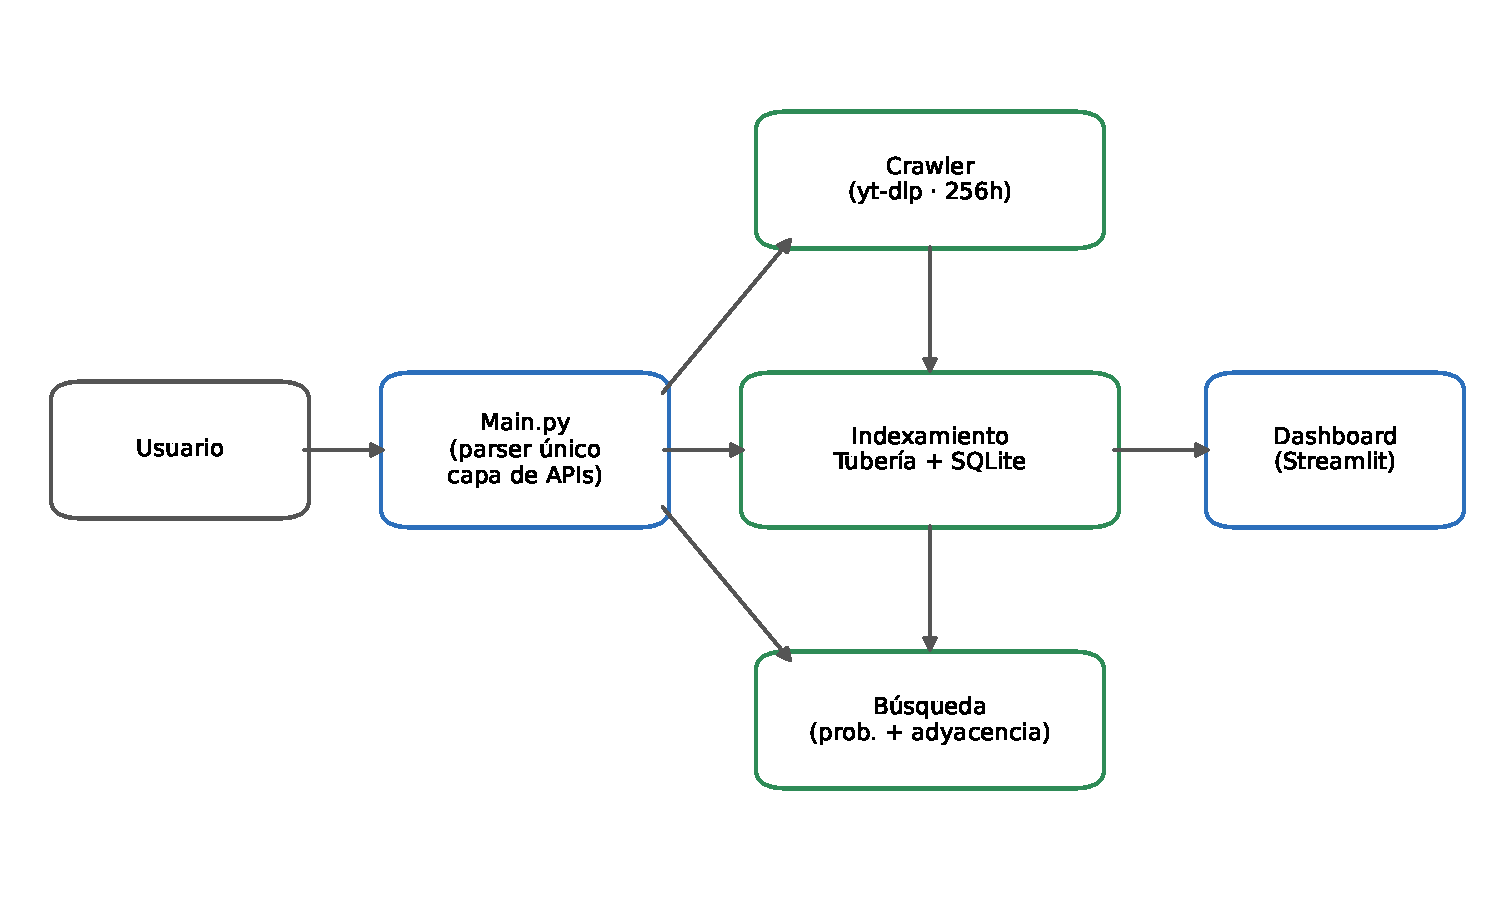
\includegraphics[width=0.92\linewidth]{figs/arquitectura.pdf}
  \caption{Arquitectura de componentes del microservicio: el parser \'unico
  (capa de \ac{API}) gobierna los servicios de Crawler, Indexamiento y
  B\'usqueda, y el panel consume la base de datos.}
  \label{fig:arq}
\end{figure}

\begin{table}[H]
  \centering
  \caption{Capa de \ac{API}: subcomandos del parser \'unico.}
  \label{tab:comandos}
  \begin{tabular}{@{}lll@{}}
    \toprule
    Subcomando & Servicio & Funci\'on \\
    \midrule
    \texttt{Retrieve} & Indexamiento & ejecuta la tuber\'ia completa \\
    \texttt{List}     & Indexamiento & inspecciona la tuber\'ia (lista URLs) \\
    \texttt{Buscar}   & B\'usqueda   & consulta probabil\'istica de campos \\
    \texttt{Crawl}    & Crawler      & prueba el crawler de forma aislada \\
    \texttt{Dashboard}& Indexamiento & lanza el panel Streamlit \\
    \bottomrule
  \end{tabular}
\end{table}

% ---------------------------------------------------------------------
\subsection{Arquitectura de Indexamiento (tuber\'ia)}\label{ssec:index}

El servicio de Indexamiento aplica el patr\'on arquitect\'onico de
\emph{tuber\'ia} (pipe--filter): la informaci\'on fluye por una secuencia de
filtros independientes (Figura~\ref{fig:tuberia}). El primer filtro,
\textbf{Crawler}\label{ssec:crawler}, descubre las URLs del canal y descarga
los metadatos, los comentarios, la miniatura (codificada en base64) y el video
escalado a 256~p\'ixeles de alto; los filtros siguientes transcriben, resumen y
clasifican, y el \'ultimo persiste el registro en SQLite. Entre cada video la
tuber\'ia se detiene 90~segundos, y los par\'ametros \texttt{--N} y
\texttt{--Path} controlan la cantidad de videos (m\'inimo 30) y la ruta.

\begin{figure}[H]
  \centering
  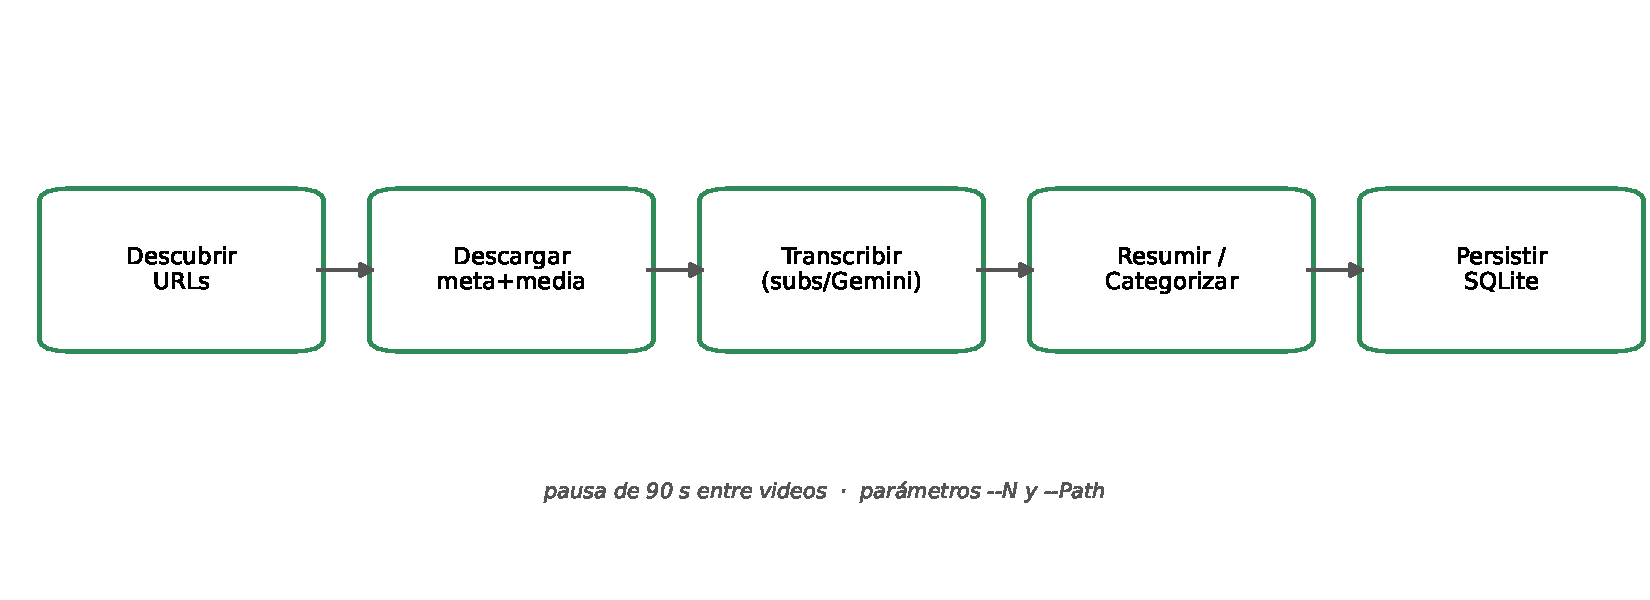
\includegraphics[width=0.95\linewidth]{figs/tuberia.pdf}
  \caption{Tuber\'ia (pipe--filter) del servicio de Indexamiento.}
  \label{fig:tuberia}
\end{figure}

El Cuadro~\ref{tab:sdd-index} resume c\'omo el dise\~no de este servicio
responde a las perspectivas del \ac{SDD} (IEEE 1016-2009). La perspectiva de
\emph{Informaci\'on} se concreta en el esquema de la base de datos
(Cuadro~\ref{tab:esquema}).

\begin{table}[H]
  \centering
  \caption{Perspectivas \ac{SDD} aplicadas a la arquitectura de Indexamiento.}
  \label{tab:sdd-index}
  \begin{tabular}{@{}p{2.6cm}p{11.5cm}@{}}
    \toprule
    Perspectiva & Concreci\'on en el dise\~no \\
    \midrule
    Contexto     & Caja negra que recibe una URL de canal y entrega una base de datos poblada. \\
    Composici\'on& Filtros: descubrir, descargar, transcribir, resumir/categorizar, persistir. \\
    L\'ogica     & M\'odulos \texttt{pipeline}, \texttt{crawler}, \texttt{enrich}, \texttt{db}. \\
    Dependencia  & El flujo es lineal; cada filtro depende solo del registro previo. \\
    Informaci\'on& Tabla \texttt{videos} en SQLite (Cuadro~\ref{tab:esquema}). \\
    Patrones     & Pipe--filter; alta cohesi\'on y bajo acoplamiento. \\
    Interfaz     & \texttt{Retrieve} y \texttt{List} en la capa de \ac{API}. \\
    Estructura   & Carpeta \texttt{indexamiento/} independiente y reutilizable. \\
    Interacci\'on& Mensajes secuenciales registro a registro, con pausa de 90~s. \\
    \bottomrule
  \end{tabular}
\end{table}

\begin{table}[H]
  \centering
  \caption{Perspectiva de Informaci\'on: esquema de la tabla \texttt{videos}.}
  \label{tab:esquema}
  \begin{tabular}{@{}lll@{}}
    \toprule
    Campo & Tipo & Descripci\'on \\
    \midrule
    \texttt{url}           & TEXT (PK) & identificador del video \\
    \texttt{captura\_ts}   & TEXT & estampa de captura (fecha y hora) \\
    \texttt{fecha\_pub}    & TEXT & fecha de publicaci\'on \\
    \texttt{duracion}      & INTEGER & duraci\'on en segundos \\
    \texttt{views, likes}  & INTEGER & reacci\'on social \\
    \texttt{n\_comentarios}& INTEGER & n\'umero de comentarios \\
    \texttt{comentarios}   & TEXT & comentarios en \ac{JSON} \\
    \texttt{thumbnail\_b64}& TEXT & miniatura en base64 (hex64) \\
    \texttt{categoria}     & TEXT & categor\'ia (Figura~1 de la actividad) \\
    \texttt{resumen}       & TEXT & resumen del contenido \\
    \texttt{transcripcion} & TEXT & transcripci\'on \\
    \bottomrule
  \end{tabular}
\end{table}

El panel (\emph{dashboard}) responde preguntas en \ac{NL} sobre el canal y, para
cualquier respuesta, construye un mosaico de proporci\'on 1:5 (cinco columnas
por fila) a partir de las miniaturas, adem\'as de graficar las reacciones
sociales por categor\'ia.

% ---------------------------------------------------------------------
\subsection{Arquitectura de B\'usqueda (probabil\'istica)}\label{ssec:busqueda}

El servicio de B\'usqueda (Figura~\ref{fig:busqueda}) construye, para cada campo
num\'erico, su \textbf{matriz de probabilidad} como un histograma normalizado.
Dada una consulta \texttt{campo op valor} (p.\,ej.\ \texttt{Likes > 95}), la
probabilidad de la b\'usqueda se estima como la fracci\'on emp\'irica de videos
que satisfacen el predicado,
\[
  P(\text{consulta}) \;=\; \frac{1}{n}\sum_{i=1}^{n}\mathbf{1}\!\left[x_i \;\text{op}\; v\right],
\]
y a cada video se le asocia la probabilidad emp\'irica $p$ del intervalo
(\emph{bin}) en que cae su valor. Adem\'as se imprime la \textbf{matriz de
adyacencia} de las parejas de campos, definida como la correlaci\'on de Pearson
entre los campos num\'ericos. Cuando $P(\text{consulta})$ es muy baja, el
sistema advierte al usuario y sugiere un rango v\'alido $[\min,\max]$.

\begin{figure}[H]
  \centering
  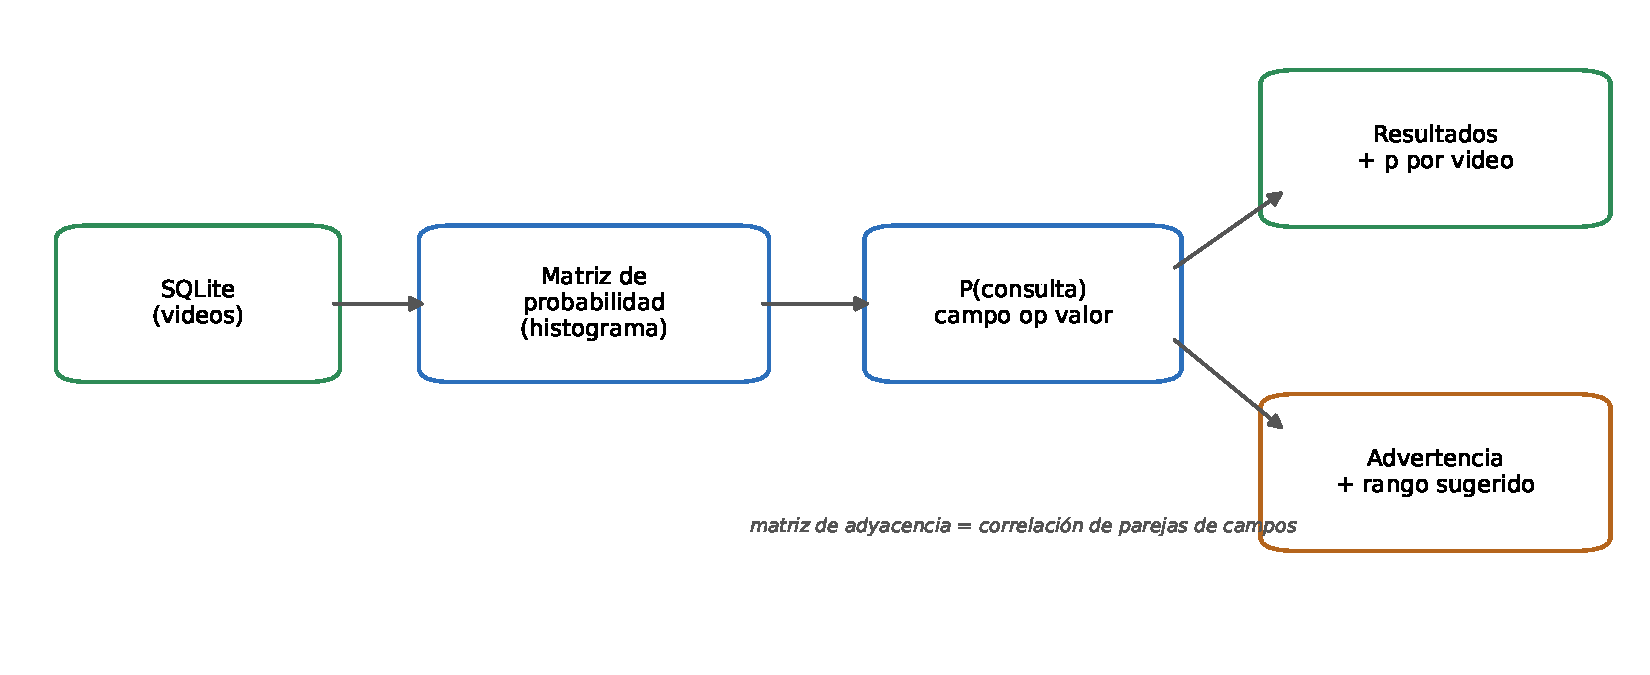
\includegraphics[width=0.95\linewidth]{figs/busqueda.pdf}
  \caption{Arquitectura del servicio de B\'usqueda probabil\'istica.}
  \label{fig:busqueda}
\end{figure}

\begin{table}[H]
  \centering
  \caption{Perspectivas \ac{SDD} aplicadas a la arquitectura de B\'usqueda.}
  \label{tab:sdd-busqueda}
  \begin{tabular}{@{}p{2.6cm}p{11.5cm}@{}}
    \toprule
    Perspectiva & Concreci\'on en el dise\~no \\
    \midrule
    Contexto     & Caja negra que recibe una consulta y entrega videos y su probabilidad. \\
    Composici\'on& Distribuci\'on por campo, evaluaci\'on del predicado y matriz de adyacencia. \\
    L\'ogica     & M\'odulo \texttt{search}: \texttt{parse\_query}, \texttt{field\_distribution}. \\
    Dependencia  & Depende \'unicamente de la tabla \texttt{videos} (lectura). \\
    Informaci\'on& Histogramas y matriz de correlaci\'on derivados de los datos. \\
    Patrones     & Validaci\'on probabil\'istica; gu\'ia al usuario. \\
    Interfaz     & \texttt{Buscar --Query "Likes > 95"} en la capa de \ac{API}. \\
    Estructura   & Carpeta \texttt{busqueda/} independiente. \\
    Interacci\'on& Consulta--respuesta con advertencia condicional. \\
    \bottomrule
  \end{tabular}
\end{table}

% =====================================================================
\section{Resultados}\label{sec:resultados}

\subsection{Back-end: llamadas a la capa de \ac{API}}

La inspecci\'on independiente de la tuber\'ia (\texttt{List}) imprime las URLs
indexadas:
\lstinputlisting[caption={Salida de \texttt{Main.py List}.}]{evidencia/list.txt}

Una b\'usqueda v\'alida imprime la probabilidad por video, la probabilidad de la
b\'usqueda y la matriz de adyacencia:
\lstinputlisting[caption={Salida de una b\'usqueda v\'alida (probabilidad alta).}]{evidencia/buscar_ok.txt}

Una b\'usqueda improbable activa la advertencia y el rango sugerido:
\lstinputlisting[caption={Salida de una b\'usqueda de baja probabilidad.}]{evidencia/buscar_low.txt}

\subsection{Front-end: operaci\'on del dashboard}

El panel (Streamlit) integra los tres servicios en cuatro pesta\~nas. La
Figura~\ref{fig:dash-nl} muestra las consultas en lenguaje natural y el mosaico
1:5; la Figura~\ref{fig:dash-busqueda}, la b\'usqueda probabil\'istica con su
matriz de adyacencia; la Figura~\ref{fig:dash-exp}, el explorador de los 30
videos; y la Figura~\ref{fig:dash-graf}, las gr\'aficas de reacci\'on social.

\begin{figure}[H]
  \centering
  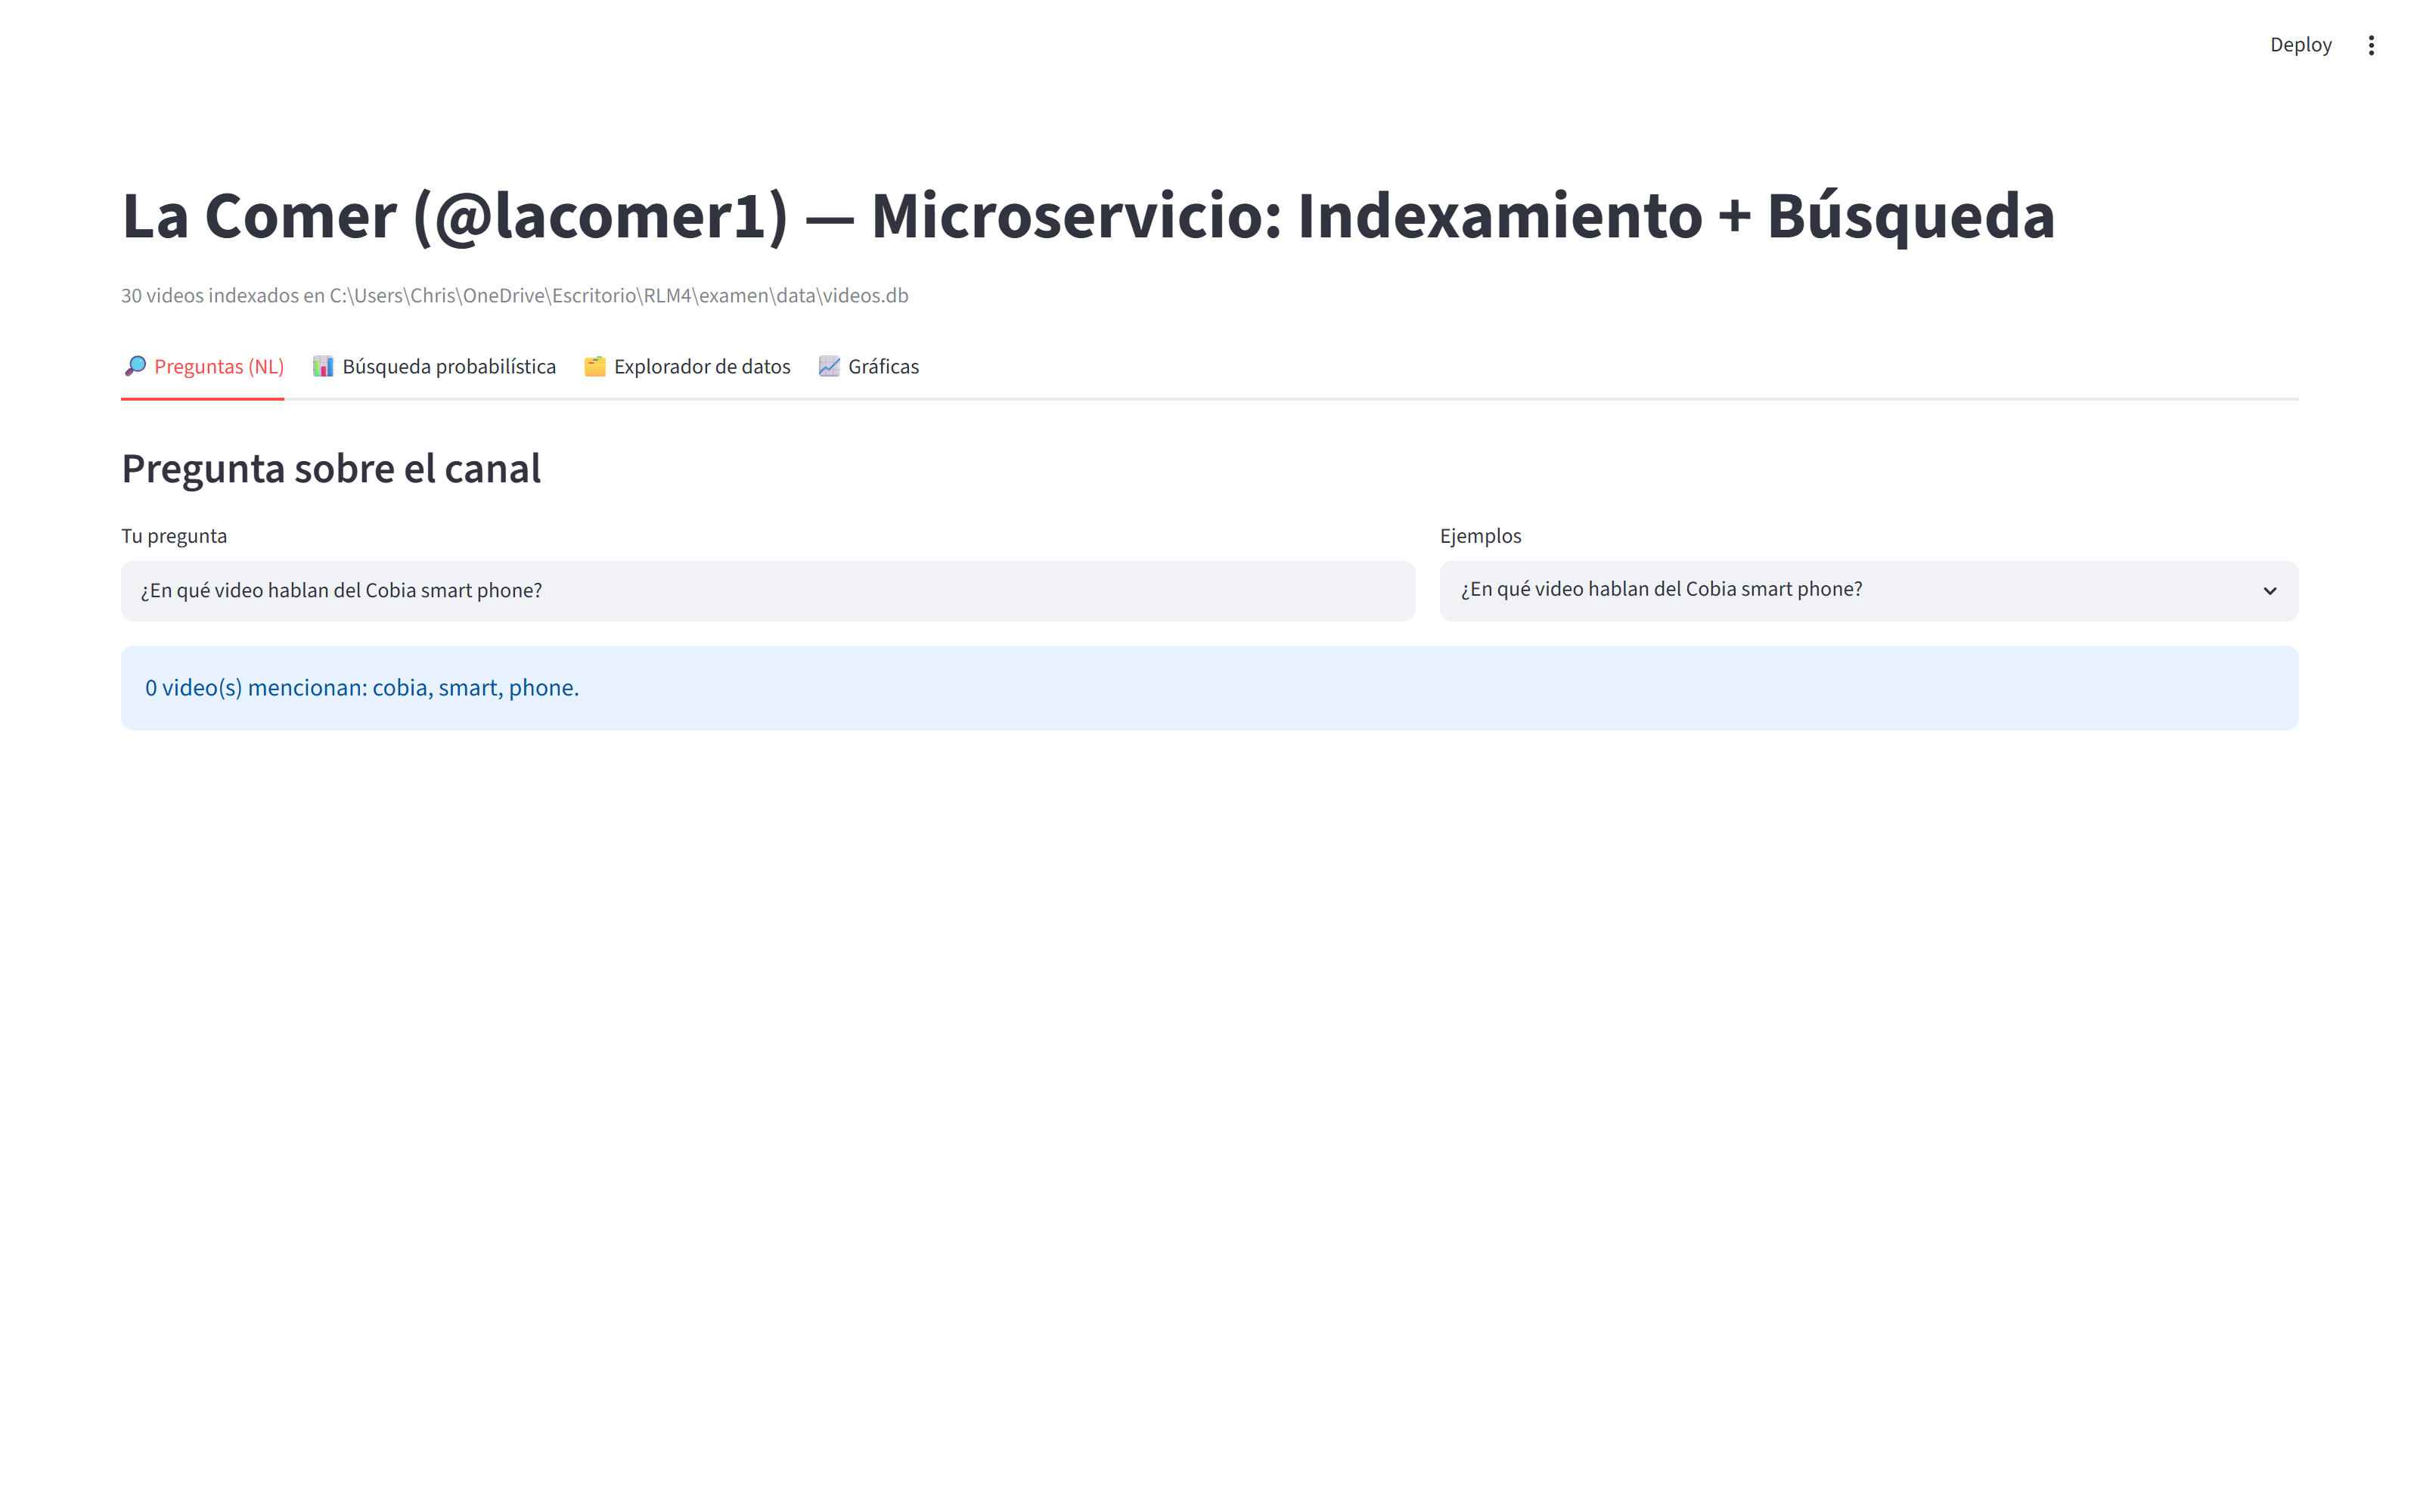
\includegraphics[width=0.95\linewidth]{figs/dash_preguntas.png}
  \caption{Dashboard: consultas en lenguaje natural y mosaico 1:5 desde los thumbnails.}
  \label{fig:dash-nl}
\end{figure}

\begin{figure}[H]
  \centering
  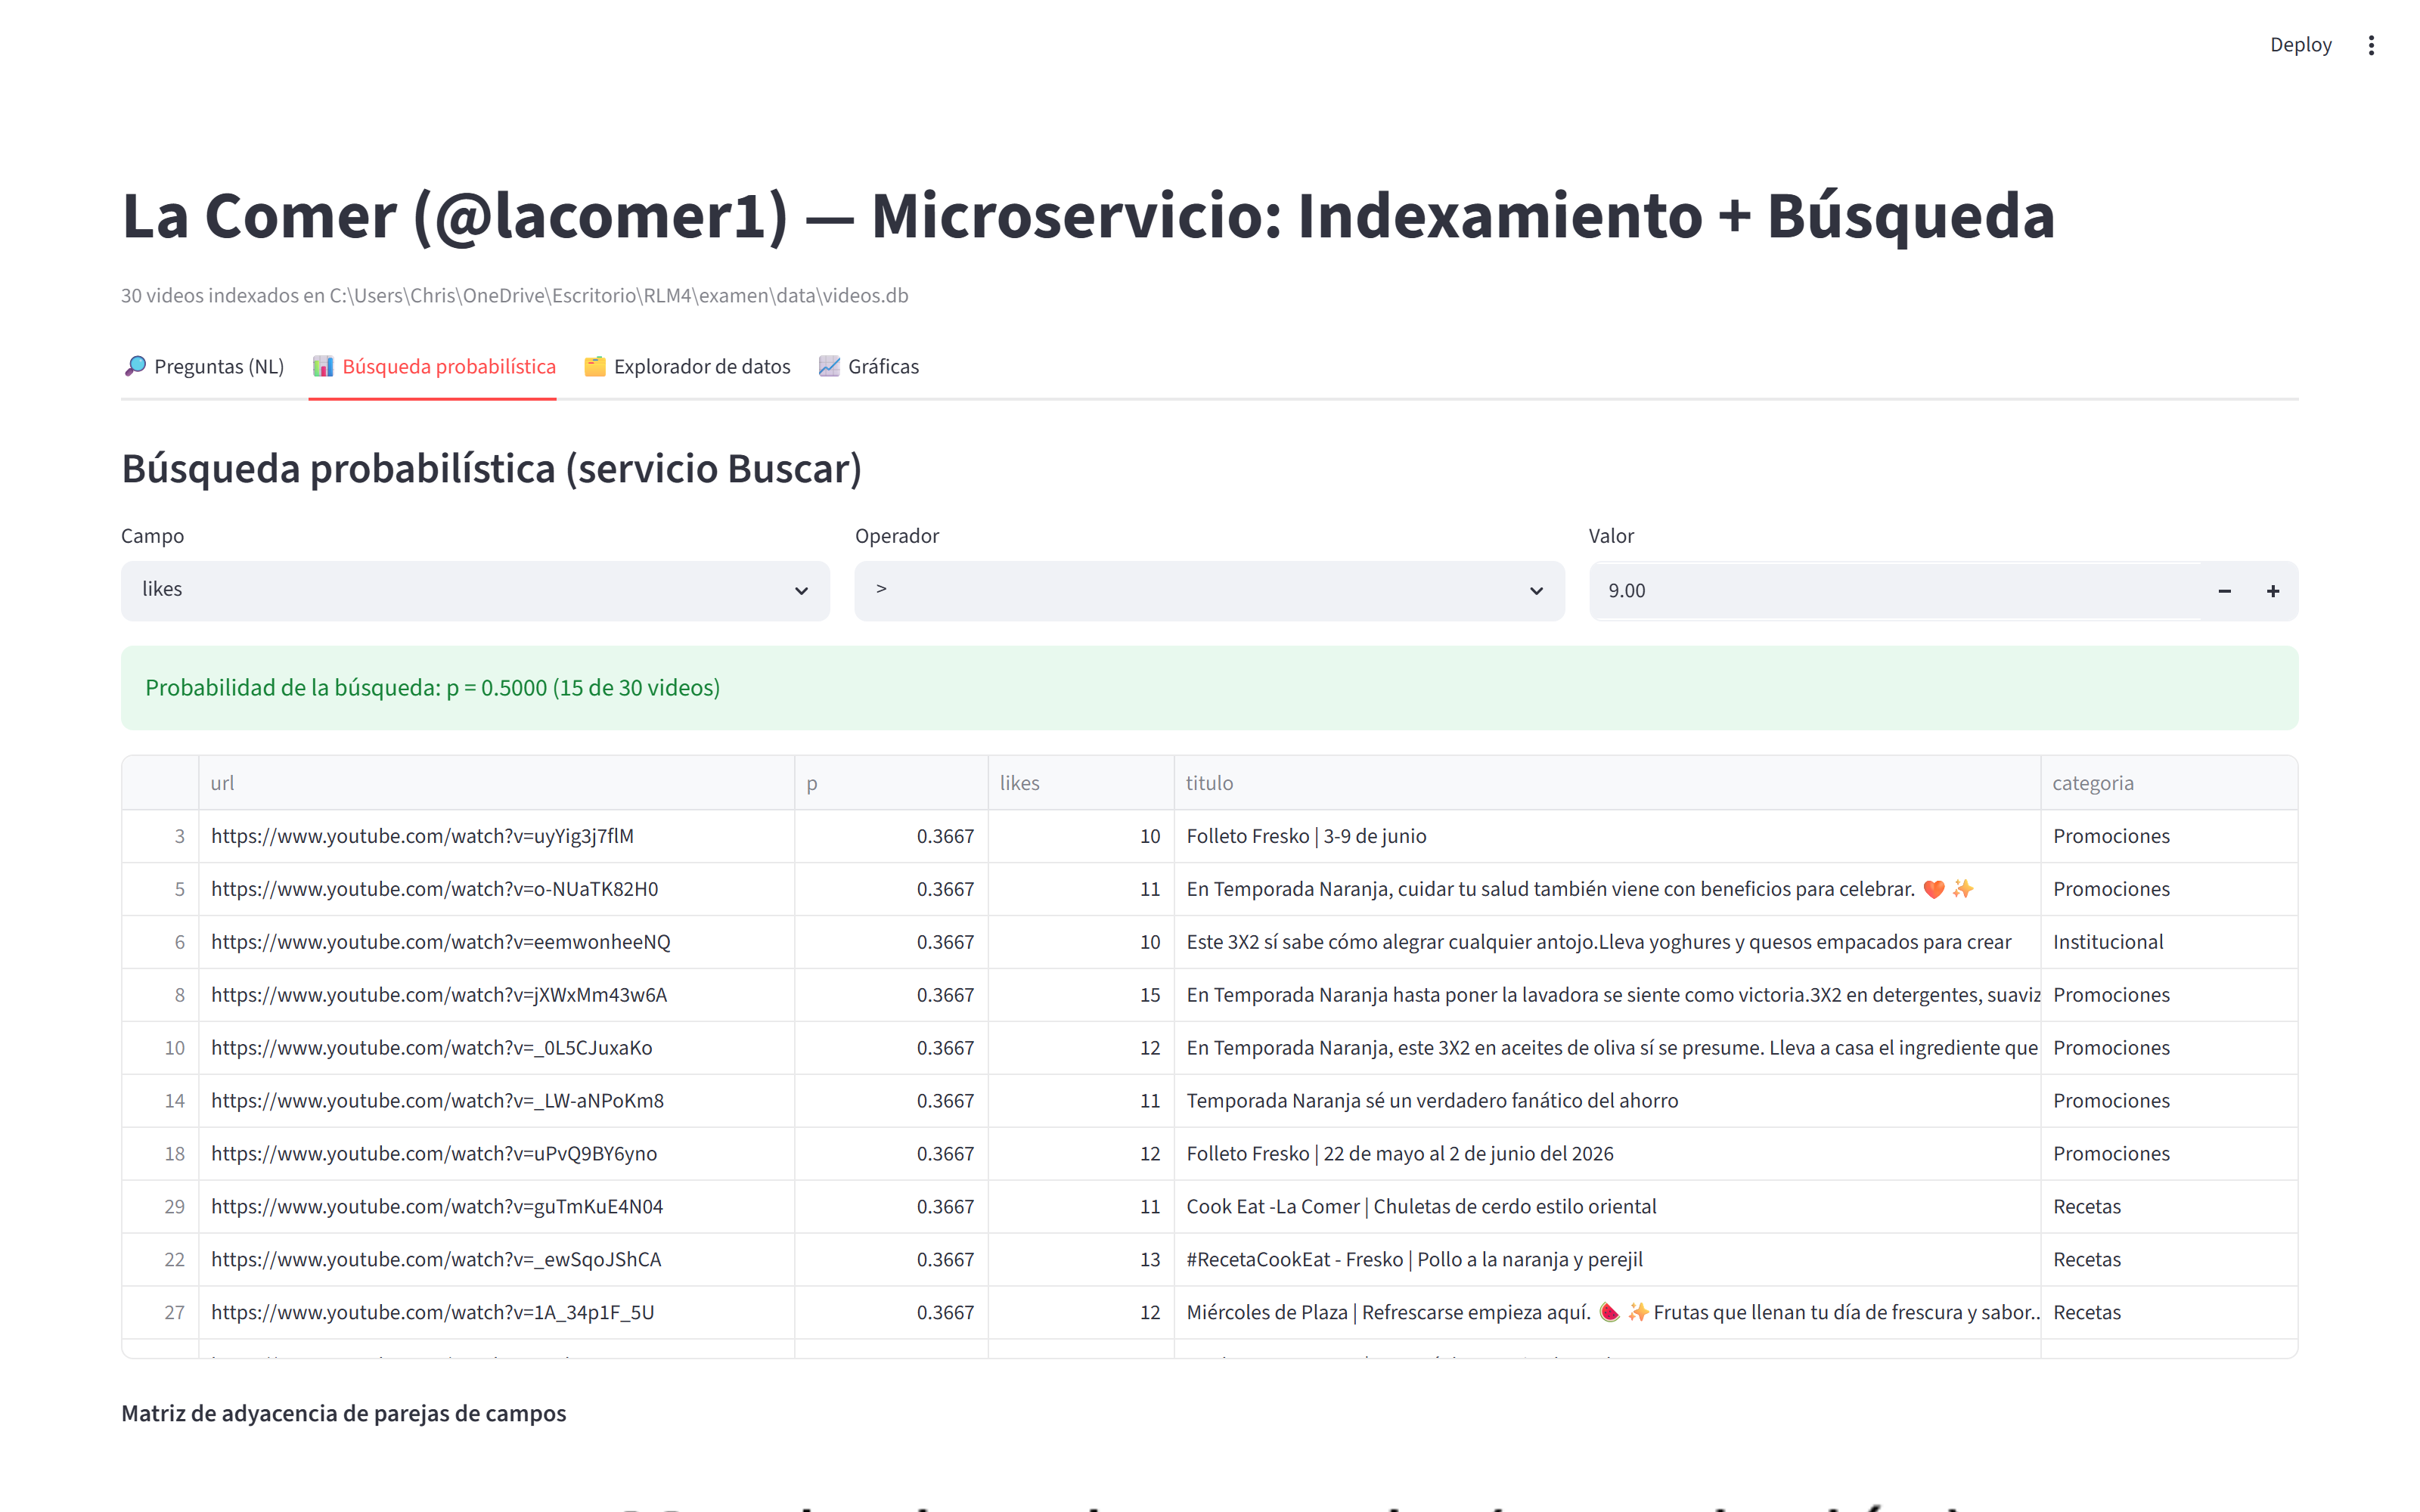
\includegraphics[width=0.95\linewidth]{figs/dash_busqueda.png}
  \caption{Dashboard: b\'usqueda probabil\'istica (servicio Buscar) y matriz de adyacencia.}
  \label{fig:dash-busqueda}
\end{figure}

\begin{figure}[H]
  \centering
  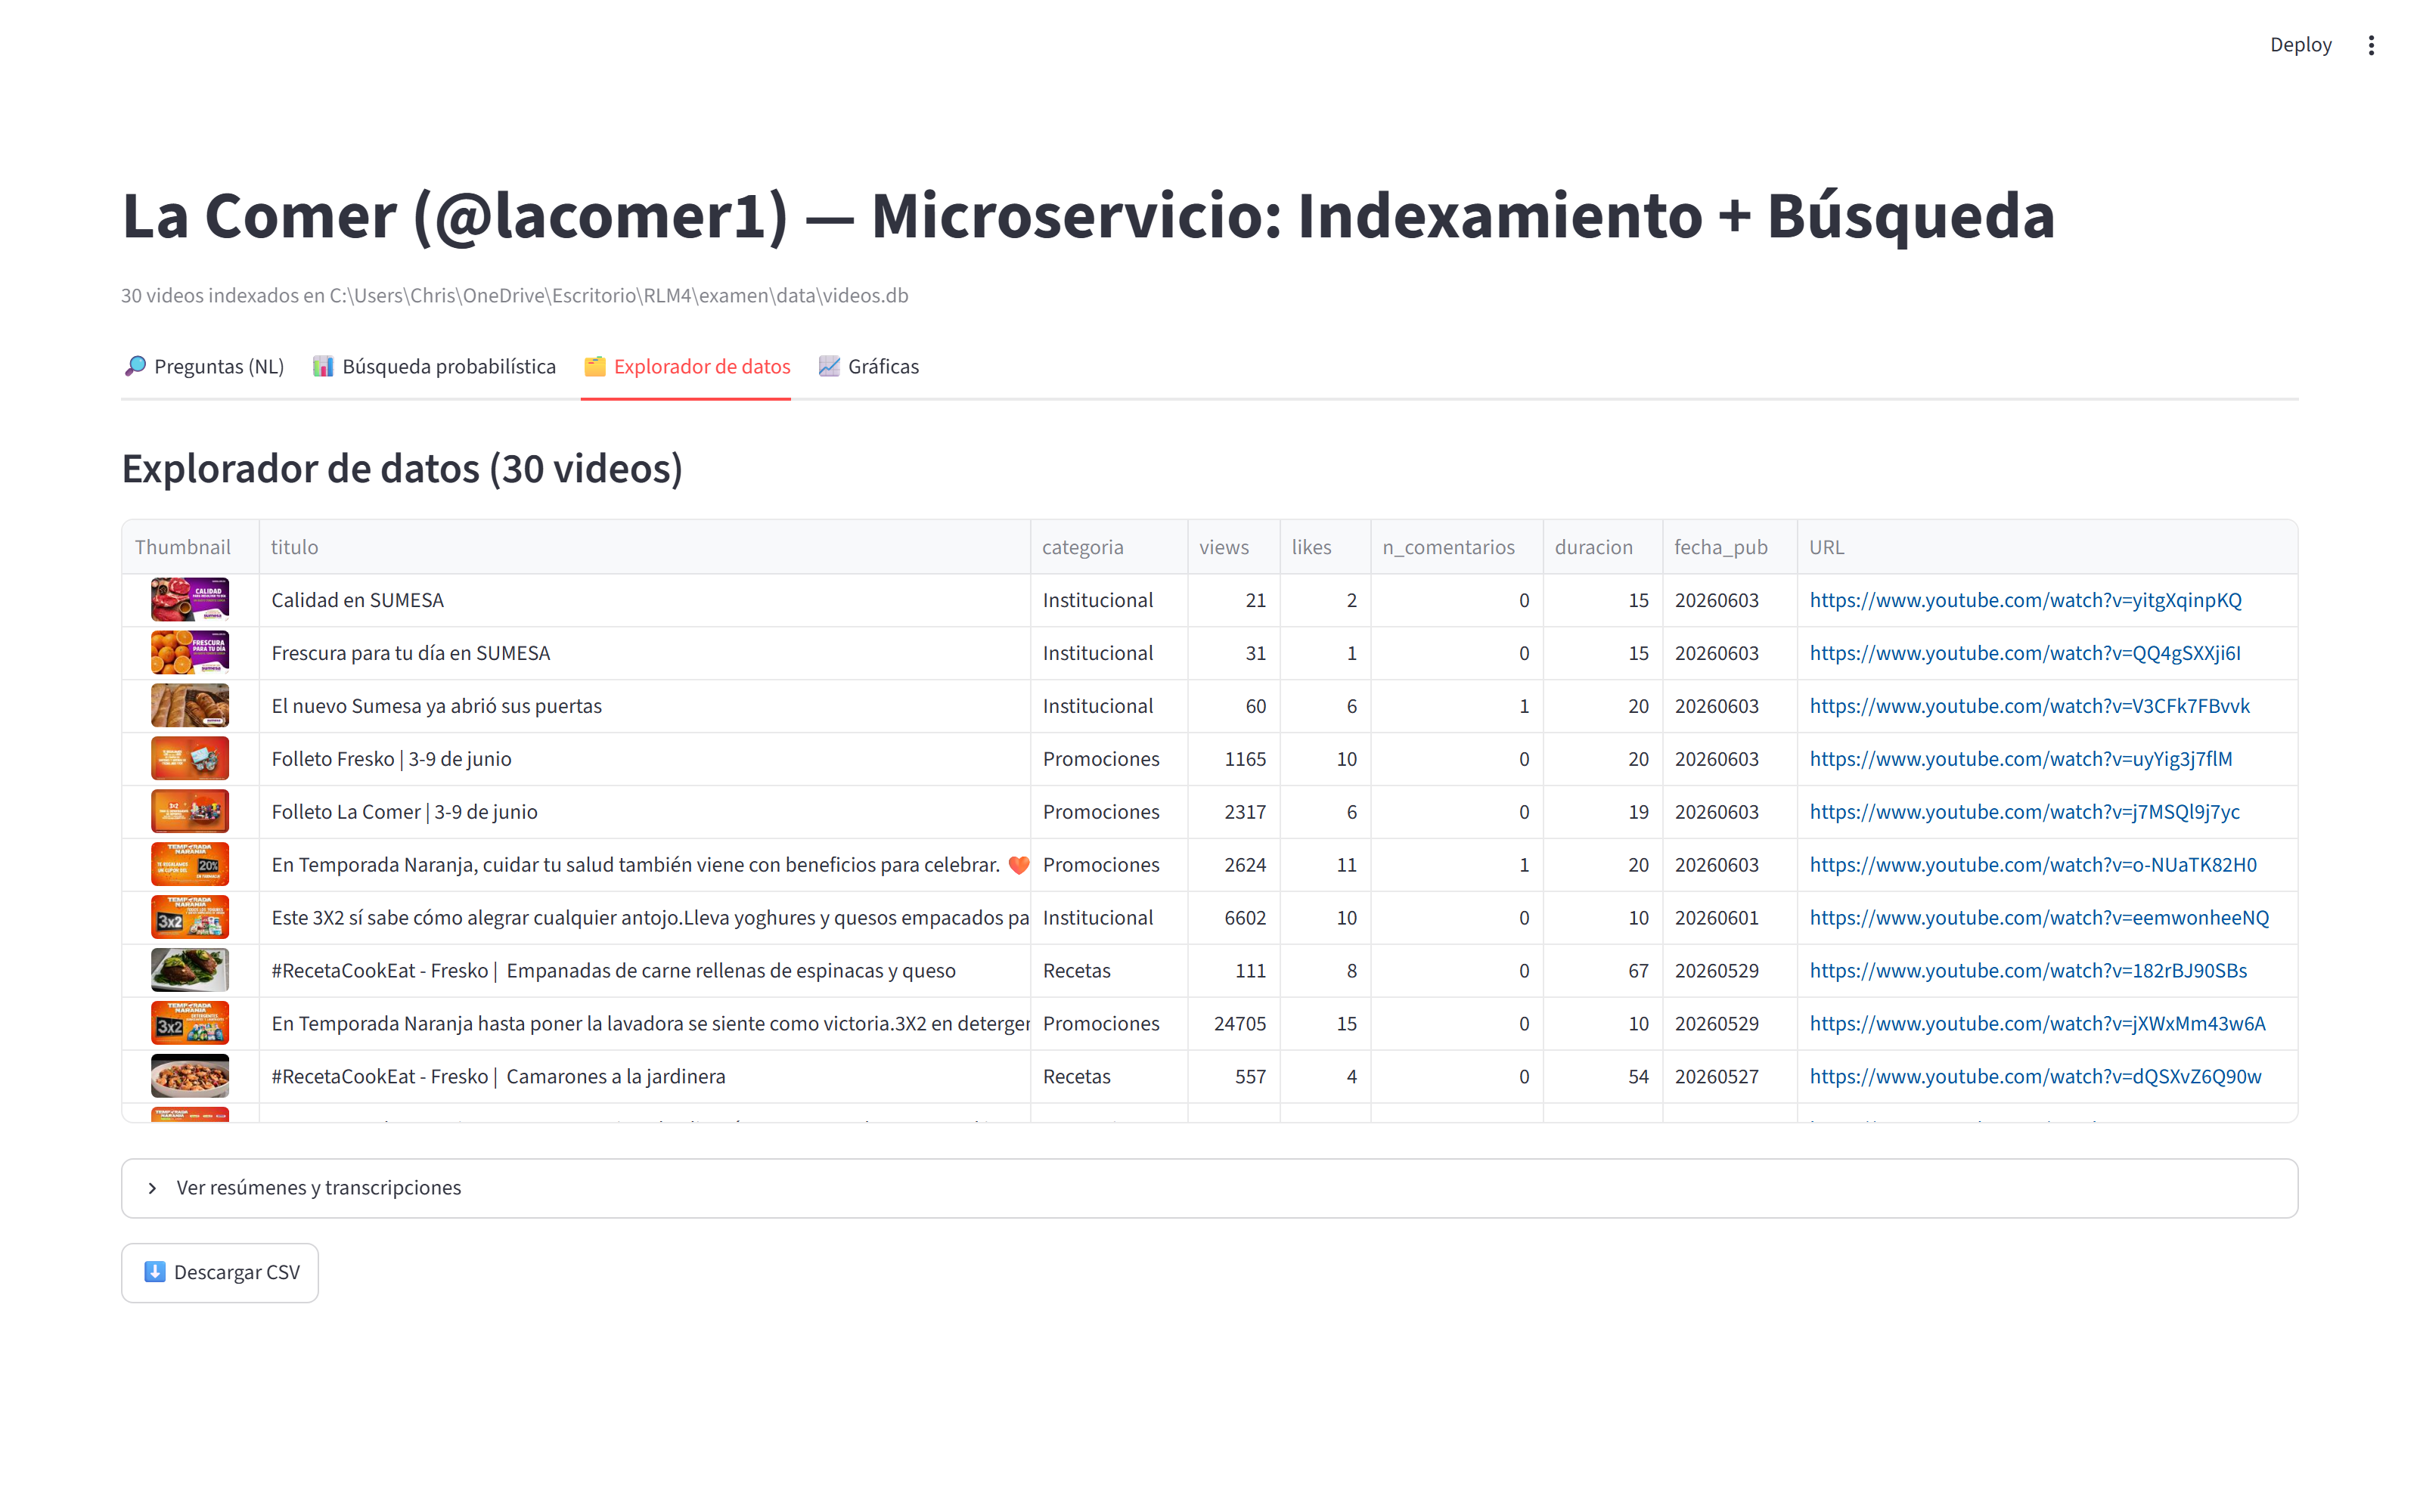
\includegraphics[width=0.95\linewidth]{figs/dash_explorador.png}
  \caption{Dashboard: explorador de los 30 videos (thumbnail, m\'etricas y descarga CSV).}
  \label{fig:dash-exp}
\end{figure}

\begin{figure}[H]
  \centering
  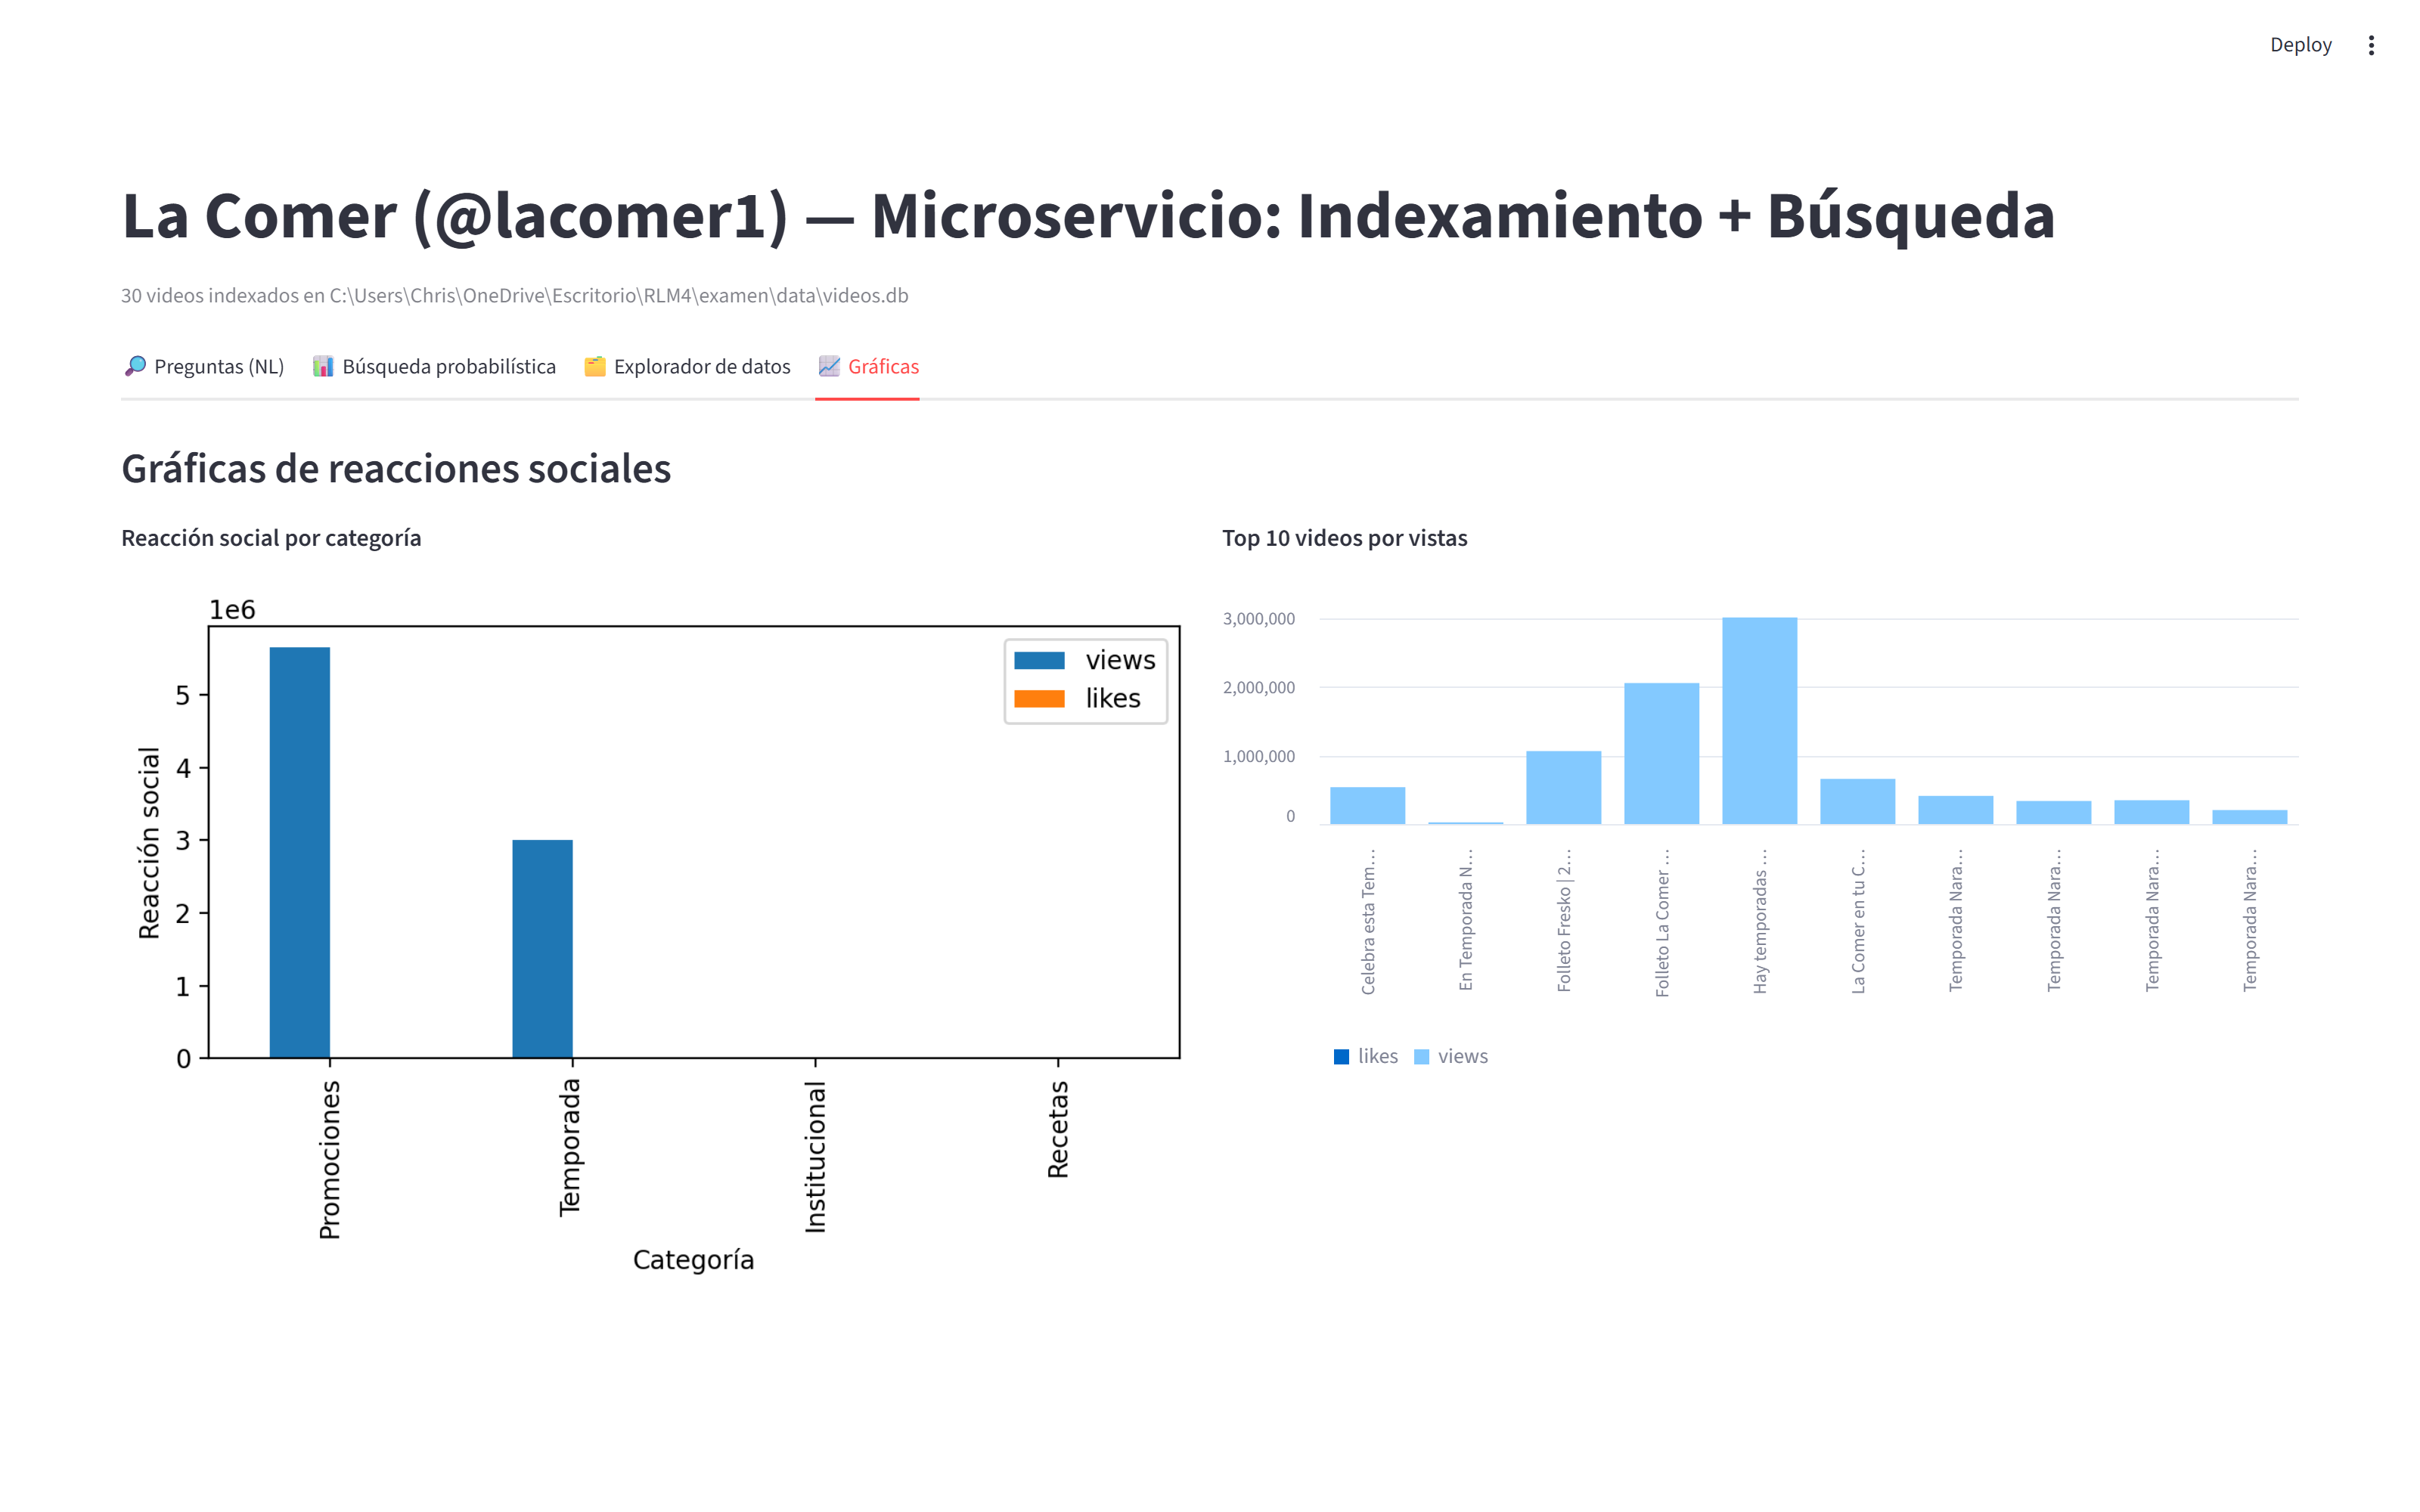
\includegraphics[width=0.8\linewidth]{figs/dash_graficas.png}
  \caption{Dashboard: gr\'aficas de reacci\'on social por categor\'ia.}
  \label{fig:dash-graf}
\end{figure}

\begin{figure}[H]
  \centering
  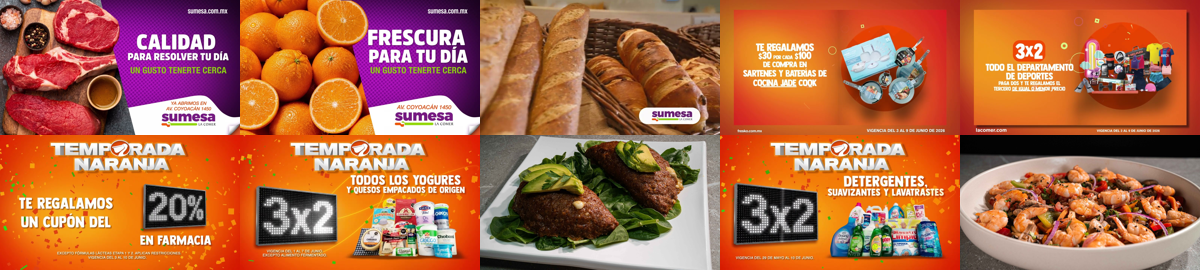
\includegraphics[width=0.95\linewidth]{figs/mosaico.png}
  \caption{Detalle del mosaico de proporci\'on 1:5 (cinco columnas por fila).}
  \label{fig:mosaico}
\end{figure}

% =====================================================================
\section{Conclusiones}\label{sec:conclusiones}
% ~250 palabras
El desarrollo confirma que separar el sistema en tres microservicios
gobernados por un \'unico \emph{parser} produce una arquitectura clara,
cohesiva y de bajo acoplamiento, tal como recomienda la teor\'ia de dise\~no y
arquitectura de software. El patr\'on de \emph{tuber\'ia} result\'o
especialmente adecuado para el Indexamiento: al modelar el procesamiento como
una secuencia de filtros independientes (descubrir, descargar, transcribir,
resumir, persistir) cada etapa puede probarse, sustituirse o reutilizarse sin
afectar a las dem\'as, y la pausa de 90~segundos se integra naturalmente en el
flujo. La capa de \ac{API}, construida con \texttt{argparse} y \emph{subparsers},
reproduce \'integramente las operaciones del sistema y permite ejercitar cada
servicio de manera aislada, lo que facilit\'o la verificaci\'on incremental. El
servicio de B\'usqueda demostr\'o el valor de un enfoque probabil\'istico: en
lugar de devolver resultados vac\'ios ante consultas imposibles, el sistema
estima la probabilidad de la consulta, advierte cuando es despreciable y sugiere
un rango v\'alido, gui\'ando al usuario hacia b\'usquedas correctas. La
especificaci\'on mediante las perspectivas del \ac{SDD} permiti\'o documentar el
dise\~no de forma sistem\'atica y vincular cada componente del diagrama con su
secci\'on correspondiente. Finalmente, la prueba din\'amica conforme a
IEEE~29119 aport\'o evidencia objetiva de robustez al ejecutar m\'as de mil
b\'usquedas autom\'aticas y registrarlas en un archivo \texttt{.out}. Como
trabajo futuro se plantea incorporar an\'alisis de sentimiento m\'as fino sobre
los comentarios, ampliar la transcripci\'on con modelos multimodales y
sustituir SQLite por un motor distribuido si el volumen de datos crece. En
conjunto, el sistema satisface los requisitos planteados y resulta mantenible y
extensible.

% =====================================================================
\section*{Glosario}
\addcontentsline{toc}{section}{Glosario}
\begin{description}[leftmargin=2.6cm,style=nextline]
  \item[Crawler] Programa que recorre autom\'aticamente un sitio para extraer informaci\'on.
  \item[Tuber\'ia (pipe--filter)] Patr\'on arquitect\'onico en el que los datos fluyen por filtros encadenados.
  \item[Matriz de probabilidad] Distribuci\'on emp\'irica (histograma normalizado) de un campo.
  \item[Matriz de adyacencia] Matriz de correlaci\'on entre parejas de campos num\'ericos.
  \item[Thumbnail] Miniatura representativa de un video.
  \item[hex64 / base64] Codificaci\'on textual de datos binarios (aqu\'i, la miniatura).
\end{description}

% =====================================================================
\appendix
\section{Ap\'endice: prueba din\'amica automatizada (IEEE~29119)}\label{ap:bash}

El siguiente \emph{script} Bash genera m\'as de mil casos de prueba aleatorios
sobre el servicio de B\'usqueda y vuelca toda la corrida al archivo
\texttt{tests/results.out}.

\lstinputlisting[language=bash,caption={\texttt{tests/auto\_test.sh}}]{auto_test.sh}

% =====================================================================
\begin{thebibliography}{9}
\bibitem{ieee1016} IEEE, ``IEEE Standard for Information Technology---Systems
Design---Software Design Descriptions,'' \emph{IEEE Std 1016-2009}, 2009.
\bibitem{ieee29119} ISO/IEC/IEEE, ``Software and systems engineering---Software
testing,'' \emph{ISO/IEC/IEEE 29119}, 2013--2022.
\bibitem{ytdlp} yt-dlp, ``A feature-rich command-line audio/video downloader,''
versi\'on 2026.03.17. [En l\'inea]. \url{https://github.com/yt-dlp/yt-dlp}
\bibitem{bs4} L. Richardson, ``Beautiful Soup Documentation.'' [En l\'inea].
\url{https://beautiful-soup-4.readthedocs.io/}
\bibitem{streamlit} Streamlit, ``A faster way to build and share data apps.''
[En l\'inea]. \url{https://streamlit.io/}
\bibitem{sqlite} SQLite, ``SQLite Documentation.'' [En l\'inea].
\url{https://www.sqlite.org/}
\bibitem{repo} C. Morales, ``Microservicio TC3005B --- C\'odigo fuente,''
repositorio GitHub. [En l\'inea].
\url{https://github.com/SinkingSeeker87/Microservicios}
\end{thebibliography}

\end{document}
